\documentclass[12pt]{ociamthesis}  % default square logo 
%\documentclass[12pt,beltcrest]{ociamthesis} % use old belt crest logo
%\documentclass[12pt,shieldcrest]{ociamthesis} % use older shield crest logo

%load any additional packages
\usepackage{amssymb}
\usepackage{listings}

\usepackage{color}
 
\definecolor{codegreen}{rgb}{0,0.6,0}
\definecolor{codegray}{rgb}{0.5,0.5,0.5}
\definecolor{codepurple}{rgb}{0.58,0,0.82}
\definecolor{backcolour}{rgb}{0.95,0.95,0.92}
 
\lstdefinestyle{mystyle}{
    backgroundcolor=\color{backcolour},   
    commentstyle=\color{codegreen},
    keywordstyle=\color{magenta},
    numberstyle=\tiny\color{codegray},
    stringstyle=\color{codepurple},
    basicstyle=\footnotesize,
    breakatwhitespace=false,         
    breaklines=true,                 
    captionpos=b,                    
    keepspaces=true,                 
    numbers=left,                    
    numbersep=5pt,                  
    showspaces=false,                
    showstringspaces=false,
    showtabs=false,                  
    tabsize=2,
    language=python
}
 
\lstset{style=mystyle}
%input macros (i.e. write your own macros file called mymacros.tex 
%and uncomment the next line)
%\include{mymacros}

\title{Modul Praktikum \\[1ex]     %your thesis title,
        Kecerdasan Buatan}   %note \\[1ex] is a line break in the title

\author{Burhanudin Zuhri}             %your name
\college{1194008\\[5ex]
Applied Bachelor of Informatics Engineering}  %your college

%\renewcommand{\submittedtext}{change the default text here if needed}
\degree{Politeknik Pos Indonesia}     %the degree
\degreedate{Bandung 2021/2022}         %the degree date

%end the preamble and start the document
\begin{document}

%this baselineskip gives sufficient line spacing for an examiner to easily
%markup the thesis with comments
\baselineskip=18pt plus1pt

%set the number of sectioning levels that get number and appear in the contents
\setcounter{secnumdepth}{3}
\setcounter{tocdepth}{3}


\maketitle                  % create a title page from the preamble info
\include{section/dedication}        % include a dedication.tex file
\include{section/acknowlegements}   % include an acknowledgements.tex file
\include{section/abstract}          % include the abstract

\begin{romanpages}          % start roman page numbering
\tableofcontents            % generate and include a table of contents
\listoffigures              % generate and include a list of figures
\end{romanpages}            % end roman page numbering

%now include the files of latex for each of the chapters etc
\chapter{Mengenal Kecerdasan Buatan dan Scikit-Learn}
\section{Teori}
Praktek teori penunjang yang dikerjakan :
\begin{enumerate}
\item
Definisi, Sejarah, dan Perkembangan Kecerdasan Buatan.
	
	\begin{enumerate}
		\item Definisi Kecerdasan Buatan
		\newline Kecerdasan Buatan (Artificial Intelligence) adalah salah satu cabang ilmu pada bidang komputer dalam memodelkan atau mensimulasikan kecerdasan manusia ke dalam komputer yang bertujuan memungkinkan suatu sistem untuk belajar dari pengalaman, mengumpulkan dan menyesuaikan input-input data baru, melaksanakan tugas, serta menyelesaikan permasalahan.
	
		\item Sejarah dan Perkembangan Kecerdasan Buatan
		\newline Sejarah kecerdasan buatan dimulai sejak abad 20 pada tahun 1940-1950, yaitu ditandai dengan mulai terbentuknya komputer modern. Pada tahun 1943, McMulloh dan Pitts mengusulkan model matematis yang diberi nama Perceptron dari neuron di dalam otak otak manusia. Pada tahun 1950, Alan Turing dalam tulisannya yang berjudul Computing Machinery and Intelligence mengeluarkan pernyataan untuk meningkatkan pengembangan Artificial Intelligenc. Pada akhir tahun 1955 program Artifical Intelligence pertama kali muncul berkat adanya perkembangan The Logic Theorist oleh Newell dan Simon. Pada tahun 1956, para ilmuan mulai berdiskusi mengenai bidang sybernetics, matematika, algoritma dan teori jaringan dan pada tahun yang sama, McCarthy mendirikan Konferensi Dartmouth di Hanover, New Hampshire dan menemukan beberapa teori kompleks mengenai jaringan sarat dan pemikiran kreatif pada komputer. Pada tahun 1960, terjadi perkembangan pesat yaitu berupa komputer telah dapat menampung lebih banyak informasi dan lebih mudah untuk mendapat akses yang cepat dan murah. Selain itu, beberapa algoritma machine learning sudah mulai digunakan untuk menyelesaikan permasalahan spesifik. Pada tahun 1971-1990, terdapat banyak milestone yang dicapai AI yaitu seperti penggunaan speech recognition software pada Dragon Systems yang diciptakan pada Windows dan disusul dengan munculnya beberapa robol yang mengimplementasikan Artificial Intelligence seperti Deep Blue, Furby, dan RoBOt (AIBO). Pada abad 21 ini, AI terus meningkat, dan informasi seputar AI semakin banyak disebarkan dan korporat juga semakin banyak menggunakan AI untuk mengembangkan machine learning.
		
	\end{enumerate}

\item
Definisi Supervised Learning, Klasifikasi, Regresi dan Unsupervised learning. Data Set, Training Set dan Testing Set.

	\begin{enumerate}
		\item Supervised Learning
		\newline Supervised Learning merupakan sebuah pendekatan yang ditentukan berdasarkan penggunaan traning set berlabel atau labeled dataset untuk membangun sebuah model yang tingkat akurasinya dapat ditingkatkan dari waktu ke waktu. Dengan kata lain, semakin banyak model tersebut mengolah data, maka tingkat keakurasiannya akan semakin tinggi juga. Supervised learning ini juga digunakan untuk melakukan klasifikasi data atau memprediksi hasil secara akurat sesuai dengan output berdasarkan pola yang ada didalam data training dan berupa data yang memiliki label yang sudah ditentukan.
		
		\item Unsupervised Learning
		\newline Unsupervised Learning merupakan sebuah pendekatan yang ditentukan berdasarkan penggunaan traning set yang tidak berlabel yang digunakan untuk menganalisa dan juga mengelompokan kumpulan data yang tidak berlabel.  Unsupervised Learning ini juga digunakan untuk menarik kesimpulan dari dataset dan untuk mempelajari suatu data berdasarkan kedekatannya saja atau yang biasa disebut dengan clustering.
		
		\item Klasifikasi
		\newline Klasifikasi merupakan teknik untuk mengidentifikasi beberapa data yang belum berlabel untuk dikategorikan menjadi sebuah bagian dari kelas diskrit. Klasifikasi ini  mempelajari hubungan antara kumpulan variabel fitur dan variabel target.
		
		\item Regresi
		\newline Regresi merupakan suatu teknik untuk mendefinisi relasi antara dua variable maupun lebih seperti variable terikat dan variabel bebas yang bertujuan untuk menemukan suatu fungsi yang dapat memodelkan data dengan meminimalkan error atau selisih antara nilai prediksi dengan nilai yang sebenarnya.
		
		\item Data Set
		\newline Data set merupakan kumpulan data yang berisi informasi-informasi lama, dan dapat dikelola sehingga menjadi sebuah informasi baru. 
		
		\item Training Set
		\newline Training set merupakan bagian dari data set yang berfungsi untuk melatih suatu algoritma agar dapat memprediksi sesuatu atau menjalankan fungsi dari algoritma tersebut.
		
		\item Testing Set
		\newline Testing set merupakan bagian dari data set yang digunakan untuk mengetahui akurasi dan performa dari algoritma yang sudah di latih oleh training set sebelumnya.
		
	\end{enumerate}
\end{enumerate}

\newpage
\section{Instalasi}
Membuka https://scikit-learn.org/stable/tutorial/basic/tutorial.html. Dengan menggunakan bahasa yang mudah dimengerti dan bebas plagiat. 
Dan wajib skrinsut dari komputer sendiri.
\begin{enumerate}
\item
Instalasi library scikit dari anaconda, mencoba kompilasi dan uji coba ambil contoh kode dan lihat variabel explorer. Gunakan perintah ”pip install -U scikit-learn”.
	\begin{figure}[!htbp]
		\centering
		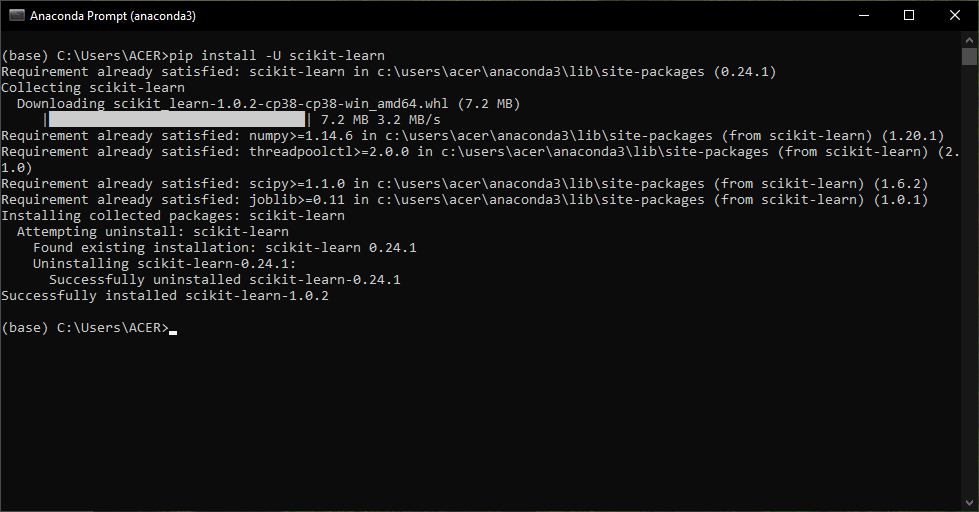
\includegraphics[scale=0.4]{figures/1.PNG}
		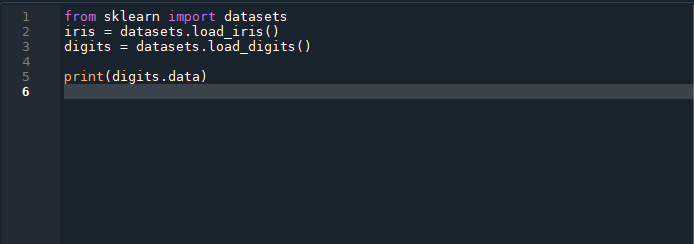
\includegraphics[scale=0.5]{figures/1a.PNG}
		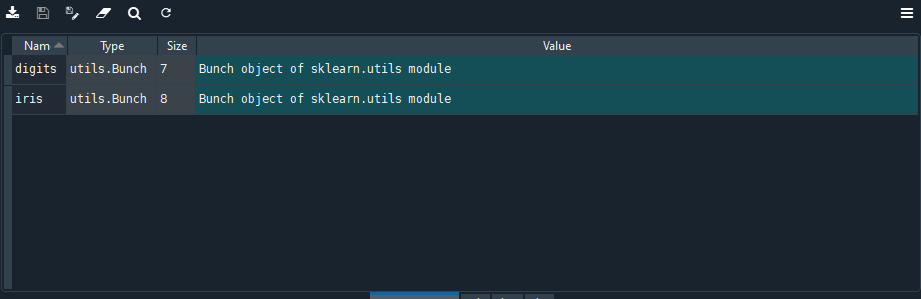
\includegraphics[scale=0.4]{figures/1b.PNG}
	\end{figure}

\newpage
\item
Mencoba Loading an example dataset, menjelaskan maksud dari tulisan tersebut dan mengartikan per baris.
	\begin{figure}[!htbp]
		\centering
		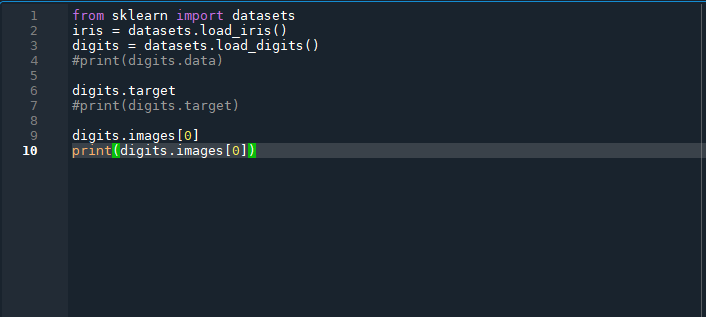
\includegraphics[scale=0.5]{figures/2.PNG}
		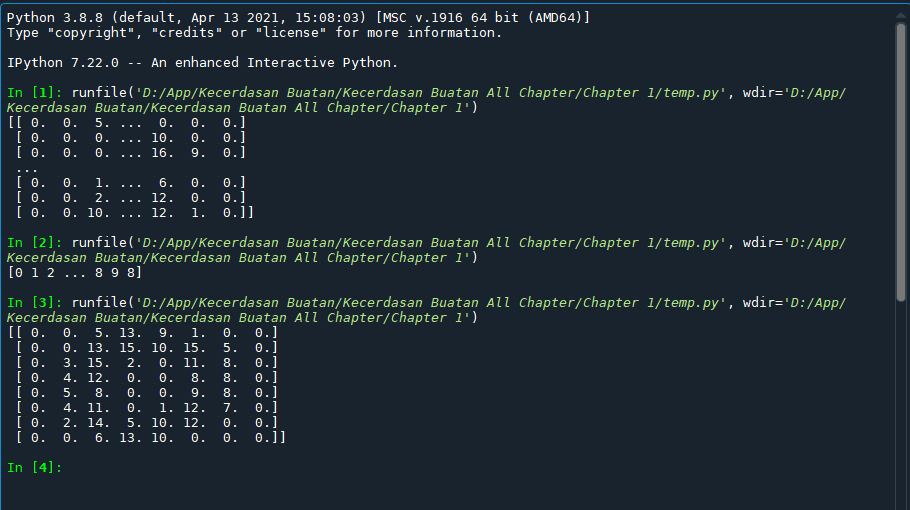
\includegraphics[scale=0.4]{figures/2a.PNG}
	\end{figure}

\newpage
\item
Mencoba Learning and predicting, menjelaskan maksud dari tulisan tersebut dan mengartikan per baris.
	\begin{figure}[!htbp]
		\centering
		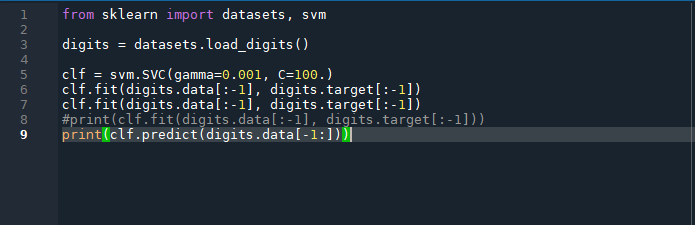
\includegraphics[scale=0.5]{figures/3.PNG}
		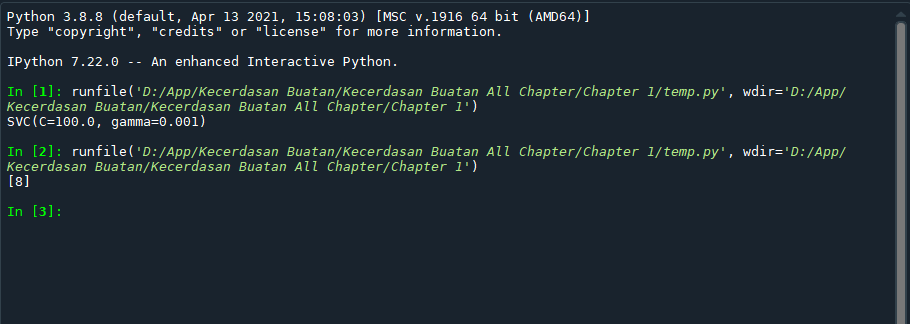
\includegraphics[scale=0.4]{figures/3a.PNG}
	\end{figure}


\item
Mencoba Model persistence, menjelaskan maksud dari tulisan tersebut dan mengartikan per baris. Terdapat dua cara yaitu menggunakan pickle atau menggunakan joblib.
	\begin{figure}[!htbp]
		\centering
		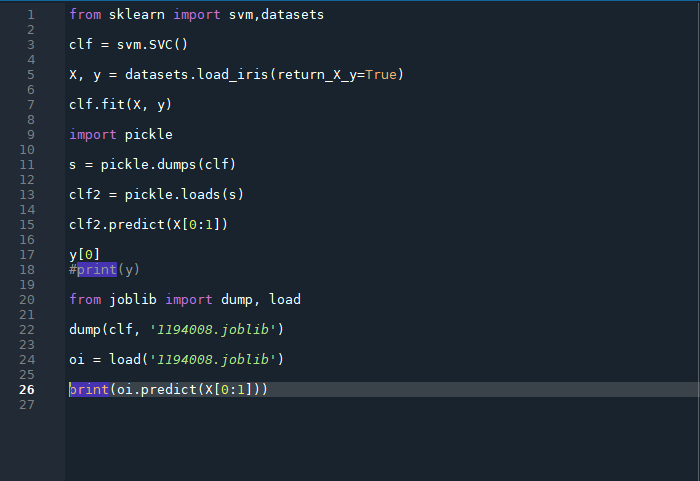
\includegraphics[scale=0.5]{figures/4.PNG}
		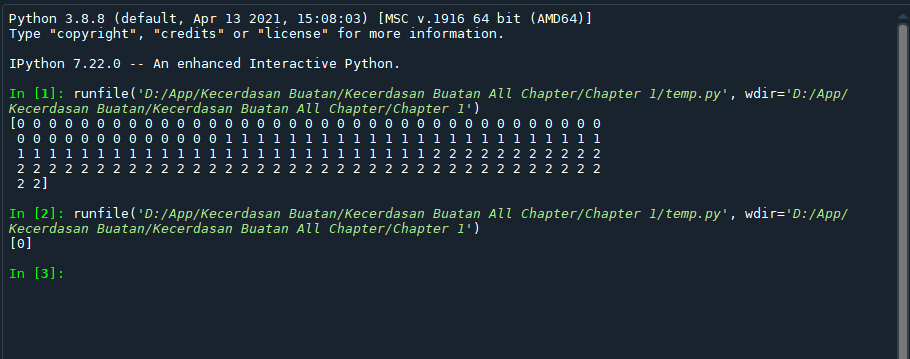
\includegraphics[scale=0.4]{figures/4a.PNG}
	\end{figure}

\newpage
\item 
Mencoba Conventions, menjelaskan maksud dari tulisan tersebut dan mengartikan per baris.
	\begin{figure}[!htbp]
		\centering
		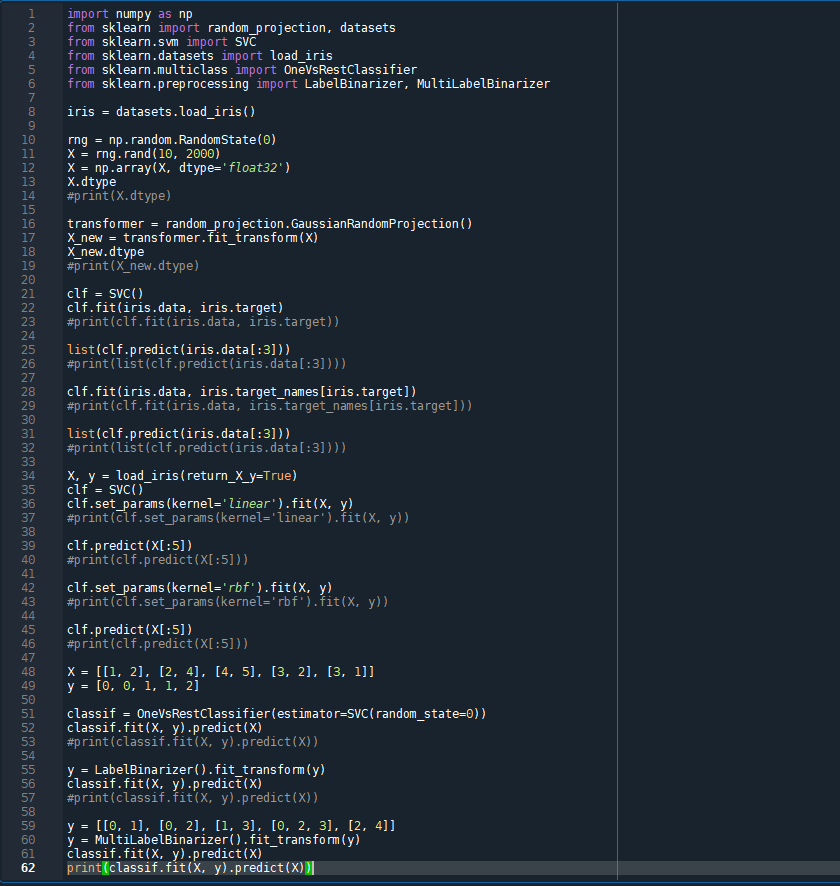
\includegraphics[scale=0.4]{figures/5.PNG}
		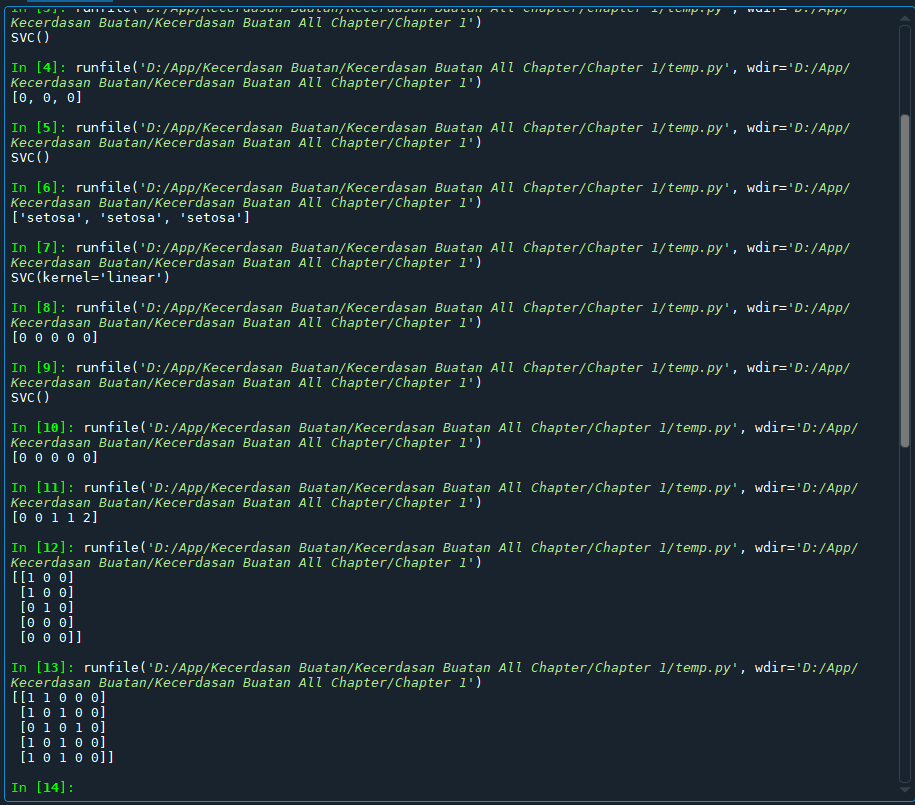
\includegraphics[scale=0.4]{figures/5a.PNG}
	\end{figure}

\end{enumerate}

\newpage
\section{Penanganan Error}
Dari percobaan yang dilakukan di atas, apabila mendapatkan error maka:

\begin{enumerate}
	\item Screenshot error.
	\begin{figure}[!htbp]
		\centering
		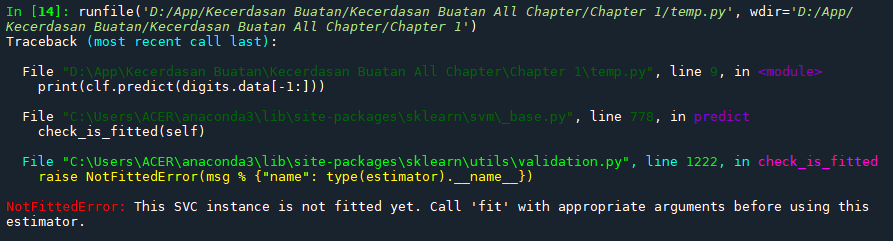
\includegraphics[scale=0.5]{figures/6.PNG}
		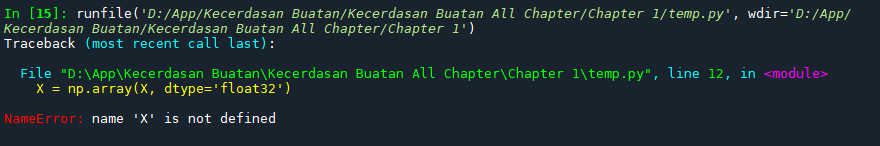
\includegraphics[scale=0.5]{figures/7.PNG}
	\end{figure}
	
	\item Tuliskan kode eror dan jenis errornya.
	\begin{enumerate}
		\item NotFittedError = This SVC instance is not fitted yet. Call ’fit’ with appropriate arguments before using this estimator.
		\item NameError = name ’X’ is not defined
	\end{enumerate}

	\item Solusi pemecahan masalah error tersebut.
	\begin{enumerate}
		\item NotFittedError = Solusinya yaitu memanggil parameter dengan method fit,
		sebelum menggunakan method predict.
		\item NameError = Solusinya yaitu membuat variabel dengan nama X.
	\end{enumerate}

\end{enumerate}


\chapter{Membangun Model Prediksi}

Untuk pratikum saati ini menggunakan buku \textit{Python Artificial Intelligence Projects for Beginners}\cite{eckroth2018python}. Dengan praktek menggunakan python 3 dan editor anaconda dan library python scikit-learn.
Dataset ada di https://github.com/PacktPublishing/Python-Artificial-Intelligence-Projects-for-Beginners .
Tujuan pembelajaran pada pertemuan pertama antara lain:
\begin{enumerate}
\item
Mengerti implementasi klasifikasi
\item
Memahami data set, training dan testing data
\item
Memahami Decission tree.
\item
Memahami information gain dan entropi.
\end{enumerate}
Tugas dengan cara dikumpulkan dengan pull request ke github dengan menggunakan latex pada repo yang dibuat oleh asisten riset. Kode program menggunakan input listing ditaruh di folder src ekstensi .py dan dipanggil ke latex dengan input listings. Tulisan dan kode tidak boleh plagiat, menggunakan bahasa indonesia yang sesuai dengan gaya bahasa buku teks.

\section{Teori}
Praktek teori penunjang yang dikerjakan(nilai 5 per nomor, untuk hari pertama) :
\begin{enumerate}
\item
Jelaskan apa itu binary classification dilengkapi ilustrasi gambar sendiri.
\newline Jawab:
\newline Binary classification merupakan proses pengklasifikasian elemen-elemen himpunan berdasarkan aturan klasifikasi yang ouputnya dibagi menjadi 2 kelompok.

\item
Jelaskan apa itu supervised learning dan unsupervised learning dan clustering dengan ilustrasi gambar sendiri.
\newline Jawab:
\newline Supervised Learning merupakan sebuah pendekatan yang ditentukan berdasarkan penggunaan
traning dataset yang berlabel/labeled dataset dan digunakan untuk melakukan klasifikasi data atau memprediksi hasil secara akurat.
\newline Unsupervised Learning merupakan sebuah pendekatan yang ditentukan berdasarkan penggunaan
traning dataset yang tidak berlabel dan digunakan untuk menganalisa serta mengelompokan kumpulan data yang tidak berlabel.
\newline Clustering merupakan sebuah proses pengelompokan data ke dalam beberapa cluster yang dimana data-data di suatu cluster tersebut memiliki kemiripan.

\item
Jelaskan apa itu evaluasi dan akurasi dari buku dan disertai ilustrasi contoh dengan gambar sendiri.
\newline Jawab:
\newline Evaluasi merupakan kegiatan untuk mengukur sebarapa baik nilai performa dari suatu
model dengan cara mengukur akurasinya. 
\newline Akurasi merupakan tigkat ketepatan yang diklasifikasikan dengan benar dari suatu model.

\item
Jelaskan bagaimana cara membuat dan membaca confusion matrix, buat confusion matrix buatan sendiri.
\newline Jawab:
\newline Cara membuat dan membaca confusion matrix:
\begin{enumerate}
	\item Menentukan studi kasusnya.
	\item Membuat ke dalam Decision Tree.
	\item Menyiapkan data testing.
	\item Mencari value dari variabel, misalnya yaitu a,b,c,d.
	\item Mencari value dari recall, precision, accuracy, dan error state.
\end{enumerate}

\item
Jelaskan bagaimana K-fold cross validation bekerja dengan gambar ilustrasi contoh buatan sendiri.
\newline Jawab:
\newline Cara kerja dari K-fold cross validation:
\begin{enumerate}
	\item Mengacak dataset secara random.
	\item Membagi dataset tersebut kedalam k-group, yaitu sebagai test dataset dan sisanya sebagai training dataset.
	\item Memasang model pada training set dan evaluasi pada test dataset.
	\item Menyimpan skor evaluasi dan buang modelnya.
	\item Meringkas keterampilan model menggunakan sampel skor menggunakan	model evaluasi.
\end{enumerate}

\item
Jelaskan apa itu decision tree dengan gambar ilustrasi contoh buatan sendiri.
\newline Jawab:
\newline Decision Tree merupakan suatu metode yang digunakan untuk membatu dalam pengambilan keputusan dengan menggunakan model pohon.

\item
Jelaskan apa itu information gain dan entropi dengan gambar ilustrasi buatan sendiri.
\newline Jawab:
\newline Information gain merupakan kumpulan informasi yang didapatkan dari variable acak.
\newline Entropi merupakan tingkat keacakan pada informasi yang diperloh dari information gain dan sedang diproses.

\end{enumerate}

\newpage
\section{scikit-learn}
Dataset ambil di https://github.com/PacktPublishing/Python-Artificial-Intelligence-Projects-for-Beginners folder Chapter01.
Tugas anda adalah, dataset ganti menggunakan \textbf{student-mat.csv} dan mengganti semua nama variabel dari kode di bawah ini dengan nama-nama makanan (NPM mod 3=0), kota (NPM mod 3=1), buah (NPM mod 3=2), . Jalankan satu per satu kode tersebut di spyder dengan menggunakan textit{Run current cell}. Kemudian Jelaskan dengan menggunakan bahasa yang mudah dimengerti dan bebas plagiat dan wajib skrinsut dari komputer sendiri masing masing nomor di bawah ini(nilai 5 masing masing pada hari kedua).

\begin{enumerate}

\item
\begin{verbatim}
	# load dataset (student mat pakenya)
	import pandas as pd
	d = pd.read_csv('student-mat.csv', sep=';')
	len(d)
\end{verbatim}
\newline Output: 
\begin{figure}[!htbp]
	\centering
	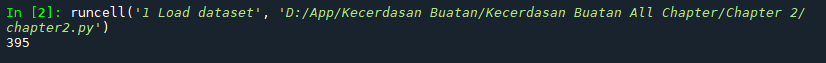
\includegraphics[scale=0.5]{figures/chapter2/1.PNG}
\end{figure}

\item
\begin{verbatim}
	# generate binary label (pass/fail) based on G1+G2+G3 
	# (test grades, each 0-20 pts); threshold for passing is sum>=30
	d['pass'] = d.apply(lambda row: 1 if (row['G1']+row['G2']+row['G3']) 
											>= 35 else 0, axis=1)
	d = d.drop(['G1', 'G2', 'G3'], axis=1)
	d.head()
\end{verbatim}
\newline Output: 
\begin{figure}[!htbp]
	\centering
	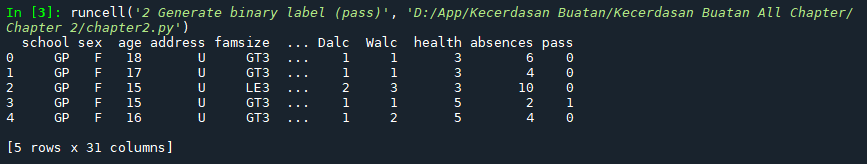
\includegraphics[scale=0.5]{figures/chapter2/2.PNG}
\end{figure}

\item
\begin{verbatim}
	# use one-hot encoding on categorical columns
	d = pd.get_dummies(d, columns=['sex', 'school', 'address', 
									'famsize', 
									'Pstatus', 'Mjob', 'Fjob', 
	                               'reason', 'guardian', 'schoolsup', 
								   'famsup', 'paid', 'activities',
	                               'nursery', 'higher', 'internet', 
									'romantic'])
	d.head()
\end{verbatim}
\newline Output: 
\begin{figure}[!htbp]
	\centering
	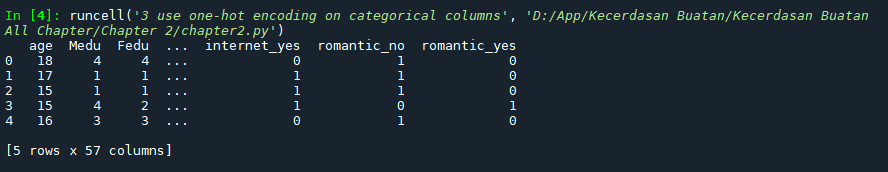
\includegraphics[scale=0.5]{figures/chapter2/3.PNG}
\end{figure}

\item
\begin{verbatim}
	# shuffle rows
	d = d.sample(frac=1)
	# split training and testing data
	d_train = d[:500]
	d_test = d[500:]

	d_train_att = d_train.drop(['pass'], axis=1)
	d_train_pass = d_train['pass']

	d_test_att = d_test.drop(['pass'], axis=1)
	d_test_pass = d_test['pass']

	d_att = d.drop(['pass'], axis=1)
	d_pass = d['pass']

	# number of passing students in whole dataset:
	import numpy as np
	print("Passing: %d out of %d (%.2f%%)" % (np.sum(d_pass), len(d_pass), 
	       100*float(np.sum(d_pass)) / len(d_pass)))
\end{verbatim}
\newline Output: 
\begin{figure}[!htbp]
	\centering
	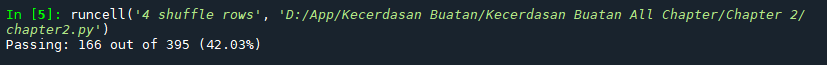
\includegraphics[scale=0.5]{figures/chapter2/4.PNG}
\end{figure}

\item 
\begin{verbatim}
	# fit a decision tree
	from sklearn import tree
	t = tree.DecisionTreeClassifier(criterion="entropy", max_depth=5)
	t = t.fit(d_train_att, d_train_pass)
\end{verbatim}
\newline Output: 
\begin{figure}[!htbp]
	\centering
	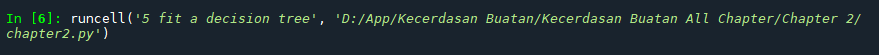
\includegraphics[scale=0.5]{figures/chapter2/5.PNG}
\end{figure}

\item
\begin{verbatim}
	# visualize tree
	import graphviz
	dot_data = tree.export_graphviz(t, out_file=None, label="all", 
									impurity=False, proportion=True,
	                                feature_names=list(d_train_att), 
									class_names=["fail", "pass"], 
	                                filled=True, rounded=True)
	graph = graphviz.Source(dot_data)
	graph
\end{verbatim}
\newline Output: 
\begin{figure}[!htbp]
	\centering
	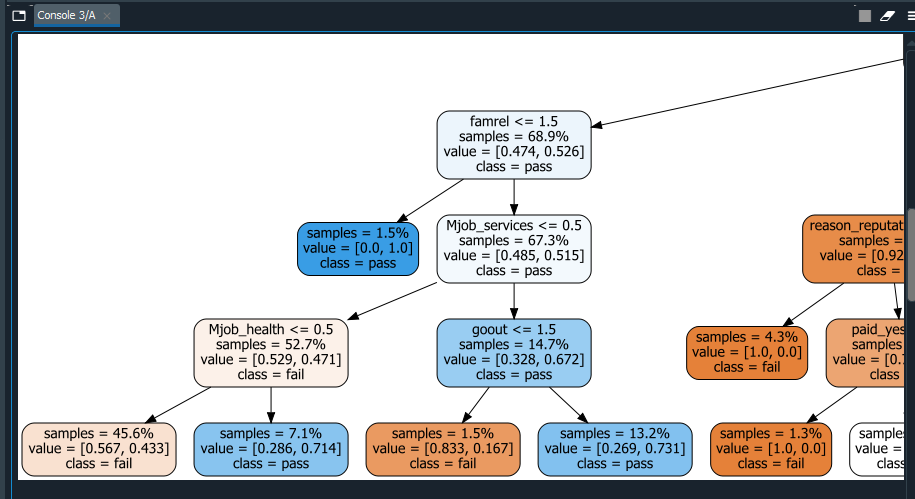
\includegraphics[scale=0.5]{figures/chapter2/6.PNG}
\end{figure}

\item
\begin{verbatim}
	# save tree
	tree.export_graphviz(t, out_file="student-performance.dot", 
						 label="all", impurity=False, 
						 proportion=True,
	                     feature_names=list(d_train_att), 
	                     class_names=["fail", "pass"], 
	                     filled=True, rounded=True)
\end{verbatim}
\newline Output: 
\begin{figure}[!htbp]
	\centering
	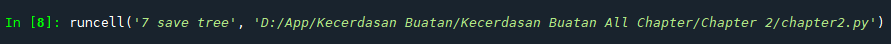
\includegraphics[scale=0.5]{figures/chapter2/7.PNG}
\end{figure}

\item
\begin{verbatim}
	t.score(d_test_att, d_test_pass)
\end{verbatim}
\newline Output: 
\begin{figure}[!htbp]
	\centering
	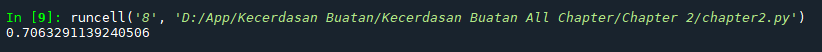
\includegraphics[scale=0.5]{figures/chapter2/8.PNG}
\end{figure}

\item
\begin{verbatim}
	from sklearn.model_selection import cross_val_score
	scores = cross_val_score(t, d_att, d_pass, cv=5)
	# show average score and +/- two standard deviations away 
	#(covering 95% of scores)
	print("Accuracy: %0.2f (+/- %0.2f)" % (scores.mean(), scores.std() * 2))
\end{verbatim}
\newline Output: 
\begin{figure}[!htbp]
	\centering
	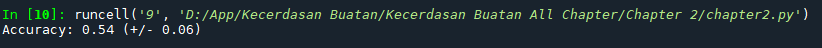
\includegraphics[scale=0.5]{figures/chapter2/9.PNG}
\end{figure}

\item 
\begin{verbatim}
	for max_depth in range(1, 20):
	    t = tree.DecisionTreeClassifier(criterion="entropy", 
			max_depth=max_depth)
	    scores = cross_val_score(t, d_att, d_pass, cv=5)
	    print("Max depth: %d, Accuracy: %0.2f (+/- %0.2f)" % 
				(max_depth, scores.mean(), scores.std() * 2)
			 )
\end{verbatim}
\newline Output: 
\newpage
\begin{figure}[!htbp]
	\centering
	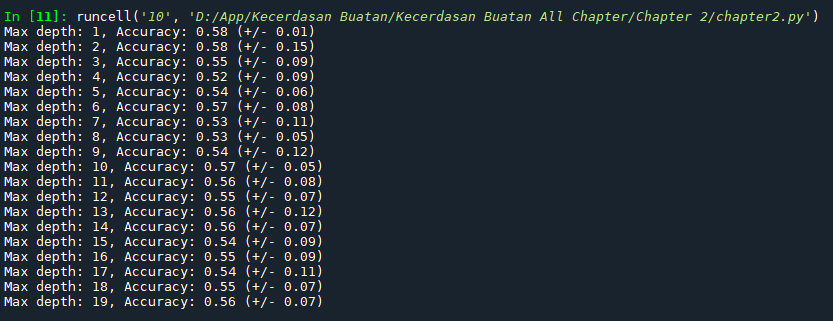
\includegraphics[scale=0.5]{figures/chapter2/10.PNG}
\end{figure}

\item
\begin{verbatim}
	depth_acc = np.empty((19,3), float)
	i = 0
	for max_depth in range(1, 20):
	    t = tree.DecisionTreeClassifier(criterion="entropy", 
			max_depth=max_depth)
	    scores = cross_val_score(t, d_att, d_pass, cv=5)
	    depth_acc[i,0] = max_depth
	    depth_acc[i,1] = scores.mean()
	    depth_acc[i,2] = scores.std() * 2
	    i += 1

	depth_acc
\end{verbatim}
\newline Output: 
\begin{figure}[!htbp]
	\centering
	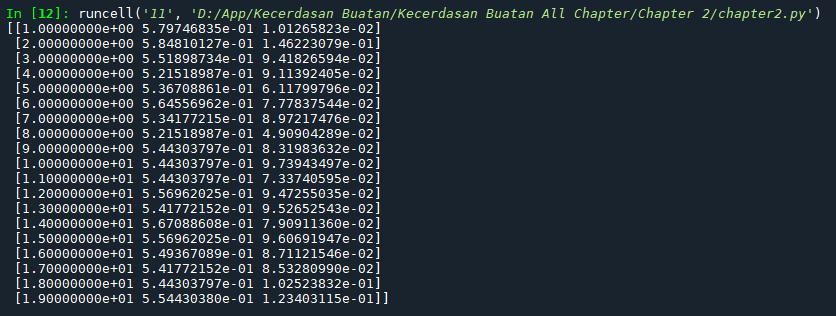
\includegraphics[scale=0.5]{figures/chapter2/11.PNG}
\end{figure}

\item 
\begin{verbatim}
	import matplotlib.pyplot as plt
	fig, ax = plt.subplots()
	ax.errorbar(depth_acc[:,0], depth_acc[:,1], yerr=depth_acc[:,2])
	plt.show()
\end{verbatim}
\newline Output: 
\begin{figure}[!htbp]
	\centering
	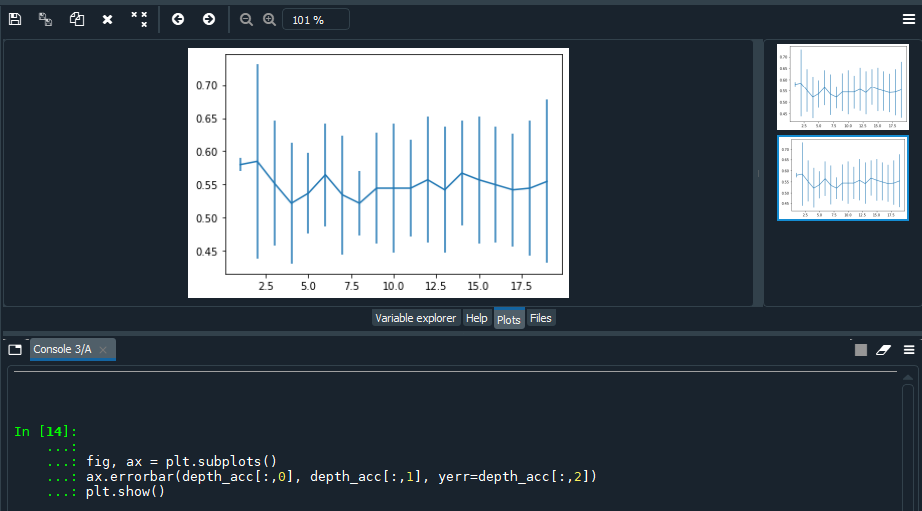
\includegraphics[scale=0.5]{figures/chapter2/12.PNG}
\end{figure}


\end{enumerate}

\newpage
\newpage
\section{Penanganan Error}
Dari percobaan yang dilakukan di atas, error yang kita dapatkan di dokumentasikan dan di selesaikan(nilai 5 hari kedua):

\begin{enumerate}
	\item Screenshot error.
	\begin{figure}[!htbp]
		\centering
		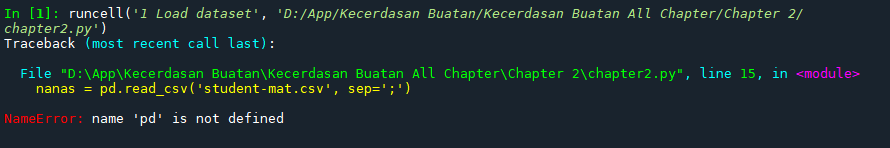
\includegraphics[scale=0.5]{figures/chapter2/13.PNG}
	\end{figure}
	
	\item Tuliskan kode eror dan jenis errornya.
	\begin{enumerate}
		\item NameError = name 'np' is not defined
	\end{enumerate}
	
	\item Solusi pemecahan masalah error tersebut.
	\begin{enumerate}
		\item NameError = Solusinya yaitu mengimport numpy dengan menginisialisaikannya sebagai np.
	\end{enumerate}
	
\end{enumerate}


%\include{section/chapter3}
%\include{section/chapter4}
%\include{section/chapter5}
%\include{section/chapter6}
%\include{section/chapter7}
%\include{section/chapter8}
%\include{section/chapter9}
%\include{section/chapter10}
%\include{section/chapter11}
%\include{section/chapter12}
%\include{section/chapter13}
%\include{section/chapter14}

%now enable appendix numbering format and include any appendices
%\appendix
%\include{section/appendix1}
%\include{section/appendix2}

%next line adds the Bibliography to the contents page
%\addcontentsline{toc}{chapter}{Bibliography}
%uncomment next line to change bibliography name to references
%\renewcommand{\bibname}{References}
%\bibliography{references}        %use a bibtex bibliography file refs.bib
%\bibliographystyle{plain}  %use the plain bibliography style

\end{document}

